\documentclass[aspectratio=169,10pt]{beamer}
\usetheme{Madrid}
\usecolortheme{default}

% \setbeameroption{hide notes} % Only slides
%\setbeameroption{show only notes} % Only notes
\setbeameroption{show notes on second screen=right} % Both

%------------------------------------------------------------
% Required packages
%------------------------------------------------------------
\usepackage{amsmath}
\usepackage[T1]{fontenc}
\usepackage[utf8]{inputenc}
\usepackage{physics}    
\usepackage{comment}    
\usepackage{color}      
\usepackage{listings}
\usepackage{csquotes}
\PassOptionsToPackage{hyphens}{url}
\usepackage{hyperref}
\usepackage{graphicx}
\usepackage{lmodern}
\usepackage{tabularx}
\usepackage{booktabs}
\usepackage{tikz}

\graphicspath{ {../figures/} }

\usetikzlibrary{arrows.meta, positioning, shapes.geometric}

% Current section
% \AtBeginSection[ ]
% {
% \begin{frame}{Outline}
%     \tableofcontents[currentsection]
% \end{frame}
% }

%------------------------------------------------------------
% Bibliography setup (using biblatex)
% Assumes 'references.bib' is in the parent directory
%------------------------------------------------------------
\usepackage[style=numeric,backend=biber]{biblatex}
\addbibresource{../references.bib}
% \renewcommand*{\bibfont}{\small}

%------------------------------------------------------------
% Title page information
%------------------------------------------------------------
\title[Automating Course Articulation]{Automating Course Articulation:\\A Deep Metric Learning Framework Using Public Data}
\author{Mark S. Kim}
\institute[SFSU]{San Francisco State University \\ Department of Data Science and Artificial Intelligence}
\date{\today}
% First draft started 7-8-2025

%------------------------------------------------------------
% Presentation slides
%------------------------------------------------------------
\begin{document}

\section{Introduction}
% The Title Slide (Slide 1.1)
\begin{frame}
    \titlepage
\end{frame}

% The Transfer Maze (Slide 1.2)
\begin{frame}
    \frametitle{The Problem: The Transfer Maze}
    
    \begin{columns}[T] % Splits the frame into columns
        
        \begin{column}{0.6\textwidth} % Left column for text
            \begin{itemize}
                \item The process for determining course equivalency, or \textbf{articulation}, is a formidable, largely manual process that creates significant barriers for students~\cite{pardos2019}.
                
                \item In California's public system alone, articulation officers at \textbf{149 individual campuses} manually negotiate and update agreements~\cite{assistfaq, ppic, calstate, cccco}.
                
                \item This task of ``bleak combinatorics'' is inefficient, slow, and inherently intractable, struggling to keep pace with the needs of a vast and mobile student body~\cite{pardos2019}.
                
                \item This is not a niche issue; transferring between institutions has become a normative part of the modern student's academic journey~\cite{publicagenda2025}.
            \end{itemize}
        \end{column}
        
        \begin{column}{0.4\textwidth}
            
            \centering
            \includegraphics[width=\textwidth]{combinatorial_web.png}
            
        \end{column}
        
    \end{columns}
\end{frame}

% The High Cost to Students & Institutions (Slide 1.3)
\begin{frame}
    \frametitle{The High Cost to Students \& Institutions}
    
    \begin{alertblock}{Consequences of an Inefficient System}
        The administrative friction of the transfer process creates a cascade of negative consequences that fall almost entirely on students.
    \end{alertblock}
    
    \begin{columns}[T]
        \begin{column}{0.6\textwidth}
            \begin{itemize}
                \item \textbf{Significant Credit Loss:} On average, transfer students lose an estimated \textbf{43\%} of their academic credits~\cite{gao2017, publicagenda2025}.
                
                \item \textbf{Increased Time-to-Degree:} Lost credits directly delay graduation and postpone entry into the workforce~\cite{gao2017}.
                
                \item \textbf{Greater Financial Burden:} Repeating courses increases tuition costs and can exhaust a student's financial aid eligibility~\cite{gao2017, collegeopportunity2017}.
                
                \item \textbf{Reduced Student Persistence:} The frustration of the process contributes to lower graduation rates for transfer students compared to their non-transfer peers~\cite{porter1999}.
            \end{itemize}
        \end{column}
        
        \begin{column}{0.4\textwidth}
            
            \centering
            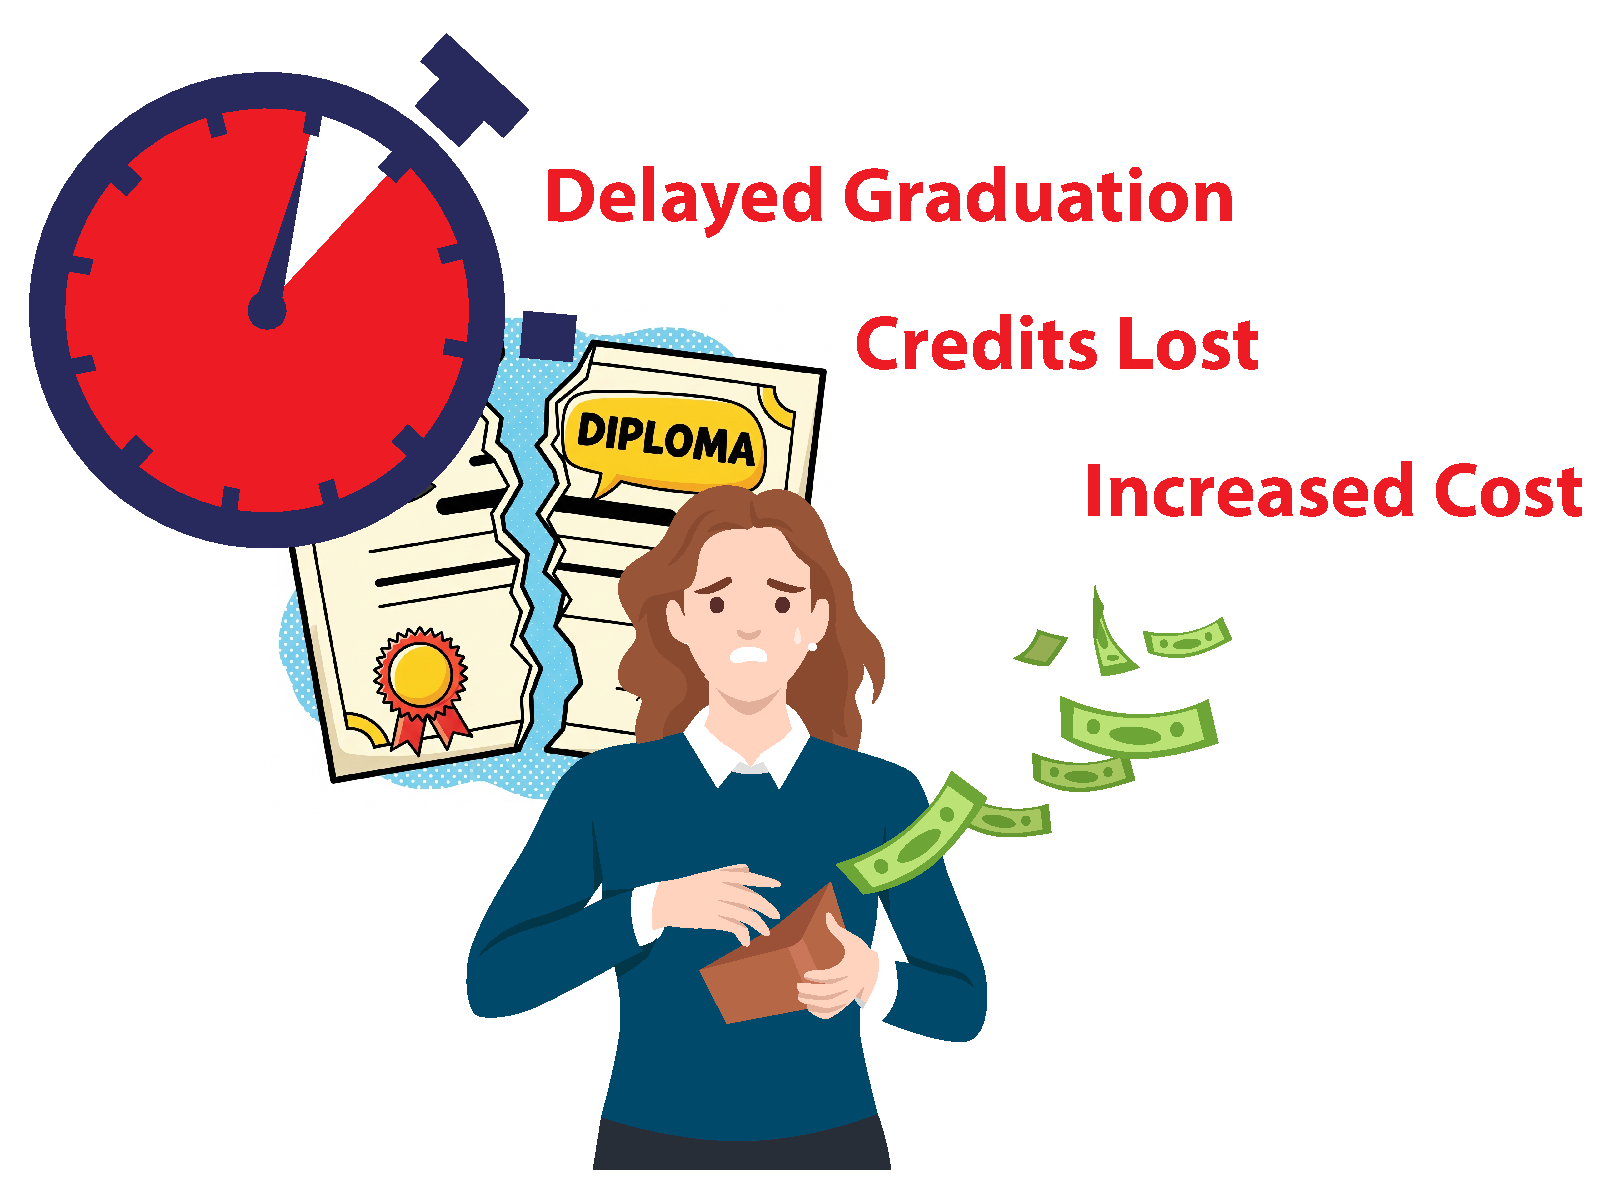
\includegraphics[width=\textwidth]{high_cost.pdf} % Placeholder for the graphic
            
        \end{column}
    \end{columns}
    
    \note[item]{This high rate of credit loss often forces students to repeat courses for which they have already received a passing grade.}
    \note[item]{This also increases their overall time in the educational system.}
    \note[item]{This means a process often undertaken to save money can paradoxically result in a greater overall financial commitment.}
    \note[item]{The frustration also has a measurable impact on student morale.}
    
\end{frame}

% A Critical Equity Issue (Slide 1.4)
\begin{frame}
    \frametitle{A Critical Equity Issue}
    
    \begin{alertblock}{This is not just an administrative problem; it's an equity problem.}
        The barriers imposed by an inefficient articulation system fall most heavily on the very students institutions are striving to support~\cite{ace2025}.
    \end{alertblock}
    
    \begin{columns}[T]
        \begin{column}{0.6\textwidth}
            \begin{itemize}
                \item Low-income and underrepresented students disproportionately rely on transfer pathways from community colleges~\cite{ace2025}.
                
                \item Recent transfer enrollment growth has been driven primarily by Black and Hispanic students~\cite{nscnews2023}.
                
                \item This creates a \textbf{feedback loop}: transfer barriers cause credit loss, imposing burdens that undermine efforts to close equity gaps~\cite{ace2025,nscnews2023}.
                
                \item Therefore, automating articulation is not just an operational optimization; it is a \textbf{necessary intervention} to foster educational equity~\cite{collegeopportunity2017}.
            \end{itemize}
        \end{column}
    
        \begin{column}{0.35\textwidth}
            
            \centering
            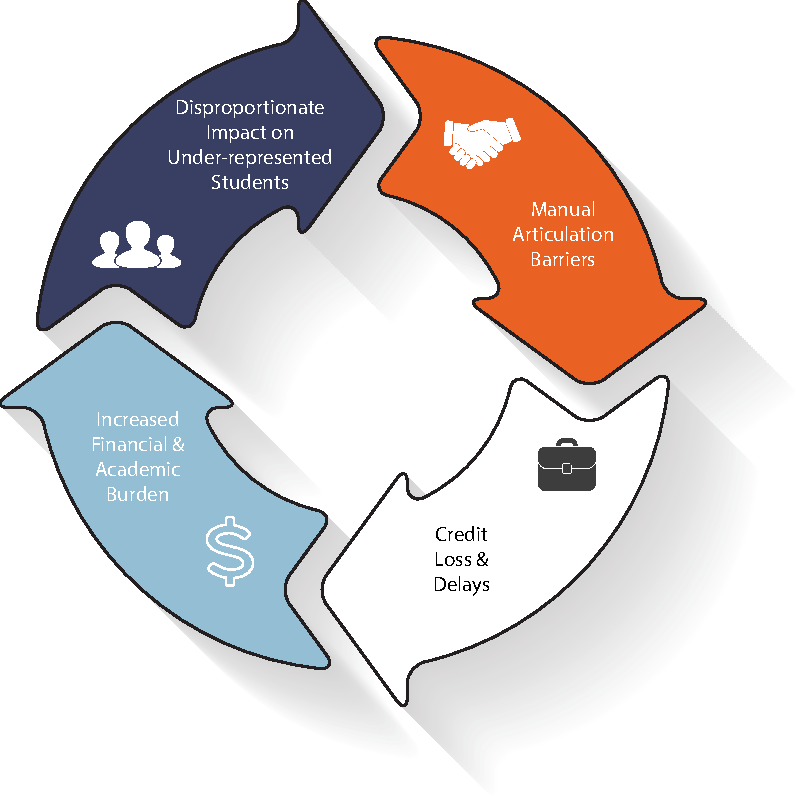
\includegraphics[width=\textwidth]{equity_issue.pdf} % Placeholder for the graphic
            
        \end{column}
    \end{columns}

    \note[item]{These are the very student populations that institutions are striving to support, making transfer efficiency a critical equity lever.}
    \note[item]{The National Student Clearinghouse reported this trend in Fall 2023, highlighting the increasing diversity of the transfer population.}
    \note[item]{This troubling loop means the manual system directly counteracts institutional goals of supporting underrepresented students.}
    
\end{frame}

% The Goal & My Contribution (Slide 1.5)
\begin{frame}
    \frametitle{The Goal \& My Contribution}
    \vspace{-0.5em}
    \begin{columns}[T]
        \begin{column}{0.47\textwidth}
            \begin{block}{The Goal}
                To develop and validate a novel framework that automates course articulation using only publicly available data.
                
                \vspace{0.5em}
                The resulting system must be:
                \begin{itemize}
                    \item<2-> Accurate \& Scalable
                    \item<3-> Computationally Efficient
                    \item<4-> Inherently Privacy-Preserving
                \end{itemize}
            \end{block}

            % --- SUGGESTED GRAPHIC ---
            % A simple diagram at the bottom of the slide could unify the concepts.
            % For example:
            % [Public Course Catalogs] -> [My Framework] -> [Accurate & Equitable Articulation]
            % This visually reinforces the input, your process, and the desired outcome.
            \begin{figure}
                \centering
                
\includegraphics[height=2.3cm]{placeholder.png} % Placeholder for the graphic
            \end{figure}

        \end{column}
        
        \begin{column}{0.47\textwidth}
            \begin{block}{Primary Contributions}
                \hfill
                \begin{enumerate}
                    \item<2-> \textbf{A Highly Accurate Framework:} Developed a complete pipeline achieving state-of-the-art accuracy on real-world data.\vspace{0.5em}
                    \item<3-> \textbf{An Innovative Feature Vector:} Designed a novel composite vector combining local and global semantics to improve classification.\vspace{0.5em}
                    \item<4-> \textbf{An Efficient \& Private Approach:} Created a decoupled solution that avoids the high costs and privacy concerns of prior methods.\vspace{1em}
                \end{enumerate}
            \end{block}
        \end{column}
    \end{columns}
    
    \note[item]{For our framework, we achieved F1-scores exceeding 0.97 on the held-out test set.}
    \note[item]{The composite vector combines the element-wise difference of course embeddings with their cosine similarity, which was shown to be a superior feature set in ablation studies.}
    \note[item]{Specifically, our approach avoids using sensitive student enrollment data and the high computational cost and opacity of direct LLM classification.}
    
\end{frame}

% % Agenda (Slide 1.6)
% \begin{frame}
%     \frametitle{Agenda}
%     \tableofcontents
% \end{frame}

% \section{Background \& Related Work}

% % The Landscape of Automation (Slide 2.1)
% \begin{frame}
%     \frametitle{The Landscape of Automation}
    
%     Prior attempts at automation have evolved, with each generation introducing new capabilities while also exposing new limitations.
    
%     \vspace{1em}

%     \footnotesize
%     \renewcommand{\arraystretch}{1.5} % Add vertical space to rows for readability
%     \begin{tabularx}{\textwidth}{>{\raggedright\arraybackslash}p{2.7cm} >{\raggedright\arraybackslash}X >{\raggedright\arraybackslash}X}
%     \toprule
%     \textbf{Approach} & \textbf{Key Characteristic} & \textbf{Core Limitation} \\
%     \midrule
    
%     Keyword \& Statistical (TF-IDF)
%     & Weight terms based on statistical importance~\cite{AIZAWA200345}.
%     & No semantic understanding; cannot grasp synonyms or context. \\
    
%     \addlinespace % Add a little extra space between rows
    
%     Static Embeddings (word2vec, GloVe)
%     & Represent words as averaged, pre-trained vectors.
%     & Context-insensitive, and averaging vectors loses critical semantic information. \\
    
%     \addlinespace
    
%     Enrollment-Based (course2vec)
%     & Learn similarity from student co-enrollment patterns~\cite{PardosCourse2Vec2019}.
%     & Requires sensitive student data, raising major privacy and generalizability issues~\cite{slade10.1177/0002764213479366}. \\
    
%     \addlinespace
    
%     Direct LLM Classification
%     & Use a large language model as an end-to-end classifier.
%     & High computational cost, opaque "black box" reasoning, and sensitive to prompt phrasing~\cite{Errica2024WhatDI}. \\
    
%     \bottomrule
%     \end{tabularx}
    
%     \note{This slide provides the full context for our work. The key takeaway is that each prior method had a significant drawback, whether it was a lack of semantic understanding, a reliance on private data, or operational complexity. This creates a clear research gap that our framework is designed to fill.}

% \end{frame}

% % The Research Gap (Slide 2.2)
% \begin{frame}
%     \frametitle{The Research Gap}
    
%     A review of prior work reveals a fundamental trade-off: as models gain semantic power, they tend to become more computationally intensive, less interpretable, or more demanding of specialized or private data.
    
%     \begin{columns}[T]
%         \begin{column}{0.4\textwidth}
%             \begin{alertblock}{The Opportunity}
%                 The limitations of direct LLM classification (cost, opacity) and enrollment-based methods (privacy, limited access) point toward a gap in the existing research for a new paradigm~\cite{pardos-articulation-2019, slade10.1177/0002764213479366}.
%                 \vspace{1em}
                
%                 \textbf{An effective solution must harness the semantic power of large models without inheriting their operational burdens.}
%             \end{alertblock}
%         \end{column}

%         \begin{column}{0.55\textwidth}
%             \begin{tikzpicture}[scale=0.9, every node/.style={transform shape}, xshift=1em]
%                 % Define styles for the boxes
%                 \tikzstyle{method} = [rectangle, rounded corners, fill=blue!10, text centered, text width=3cm]
%                 \tikzstyle{goal} = [rectangle, rounded corners, fill=green!20, text centered, text width=3cm, font=\bfseries]

%                 % Draw axes
%                 \draw[->, thick] (-3.5,0) -- (3.5,0) node[right] {\begin{tabular}{l}Cost /\\Privacy Risk\end{tabular}};
%                 \draw[->, thick] (0,-2.5) -- (0,2.5) node[above] {Semantic Power};

%                 % Place method nodes
%                 \node[method] at (-1.75, -1.25) {Keyword \& Statistical (TF-IDF)};
                
%                 \node[method] at (1.75, 1.25) {Enrollment-Based \\ Direct LLM};

%                 % Place the goal node
%                 \node[goal] at (-1.75, 1.25) {The Research Gap \\ (Our Goal)};
%             \end{tikzpicture}
%         \end{column}
%     \end{columns}

%     \note{This diagram clearly shows the trade-offs. In the bottom-left, we have simple methods with low semantic power. In the top-right, we have powerful methods that are either expensive or raise privacy concerns. The top-left quadrant is where we want to be: high semantic power, but with low cost and no privacy risk. This is the gap our research addresses.}

% \end{frame}

% \section{A Decoupled Framework for Articulation}

% \begin{frame}
%     \frametitle{Agenda}
%     \tableofcontents[currentsection]
% \end{frame}

% % High-Level Architecture (Slide 3.1)
% \begin{frame}
%     \frametitle{A Decoupled Framework: High-Level Architecture}
    
%     Our framework's core principle is to \textbf{decouple rich semantic representation from the final classification task}. This creates a more efficient, scalable, and transparent system.
    
%     \vspace{1em}
    
%     % --- SUGGESTED GRAPHIC ---
%     % A large, clear flowchart is essential for this slide. It should
%     % dominate the frame and visually walk the audience through your entire
%     % process. The flow should be:
%     %
%     % 1. Start with two boxes: "Course A Text" and "Course B Text".
%     %
%     % 2. Arrow to a box: "Deep Embedding Model". Show that this produces
%     %    "Vector A" and "Vector B".
%     %
%     % 3. Arrow to a box: "Feature Engineering". Label this process as
%     %    creating the "Composite Distance Vector (\Delta_c)".
%     %
%     % 4. Arrow to a box: "Traditional ML Classifier (e.g., SVM)".
%     %
%     % 5. Arrow to the final output: "Prediction: Equivalent / Not Equivalent".
%     %
%     % This diagram will be the clearest way to explain your entire methodology.
    
%     \begin{figure}
%         \centering
%         
\includegraphics[scale=0.25]{placeholder.png}
%     \end{figure}
    
% \end{frame}

% % Core Principle: Decoupling Representation from Classification (Slide 3.2)
% \begin{frame}
%     \frametitle{Core Principle: Decoupling Representation from Classification}

%     By separating the process into two stages, we gain the semantic power of deep learning while avoiding the high operational costs of end-to-end LLM classification~\cite{Errica2024WhatDI} and the privacy risks of enrollment-based methods~\cite{slade10.1177/0002764213479366}.
    
%     \vfill % Center the graphic vertically on the slide
%     \centering
    
%     % --- TikZ Implementation of the Flowchart ---
%     % NOTE: Ensure \usetikzlibrary{arrows.meta, positioning, shapes.geometric} is in your preamble
%     \begin{tikzpicture}[
%         node distance=1cm,
%         % Define styles for the elements
%         stage/.style={rectangle, 
%                       draw, 
%                       rounded corners,
%                       fill=blue!10, 
%                       text width=6cm, 
%                       minimum height=3.5cm, 
%                       align=center},
%         arrow/.style={-Stealth, ultra thick, draw=gray!80}
%     ]
%         % Place the nodes for each stage
%         \node (stage1) [stage] {
%             \textbf{Stage 1: Semantic Representation} \\
%             \textit{(Heavy, Offline Task)}
%             \\[2ex]
%             A deep embedding model converts raw course text into structured, reusable semantic vectors.
%         };
        
%         \node (stage2) [stage, right=of stage1] {
%             \textbf{Stage 2: Pairwise Classification} \\
%             \textit{(Lightweight, Fast Task)}
%             \\[2ex]
%             A traditional ML model performs rapid, on-demand comparisons of the pre-computed vectors.
%         };
        
%         % Draw the arrow connecting the stages
%         \draw [arrow] (stage1.east) -- (stage2.west);
        
%     \end{tikzpicture}
    
%     \vfill
    
%     \note{This is the most important concept in the framework. We do the heavy lifting of understanding language only once, offline. This lets us do the actual classification of pairs incredibly quickly and efficiently. This two-stage process is what gives us the best of both worlds: the semantic power of deep learning without the high operational costs for every comparison, which is what makes the system so scalable and practical.}
% \end{frame}

% % Step 1: Deep Contextual Embeddings (Slide 3.3)
% \begin{frame}
%     \frametitle{Step 1: Deep Contextual Embeddings}

%     The first step is to convert unstructured course catalog text into a structured, semantically rich vector using a pre-trained transformer model~\cite{devlin2019bertpretrainingdeepbidirectional, reimers-2019-sentence-bert}.
    
%     \vfill

%     \begin{figure}
%         \centering
%         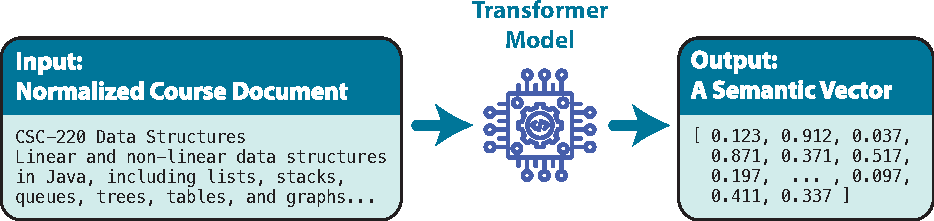
\includegraphics[width=\textwidth]{text_to_vector.pdf}
%     \end{figure}

%     \note{The key here is that we're turning unstructured text into a structured, mathematical object—a vector. We use a pre-trained transformer model for this, specifically models from the Sentence-BERT family~\cite{devlin2019bertpretrainingdeepbidirectional, reimers-2019-sentence-bert}. The resulting vector captures the actual meaning of the course, so similar courses will have vectors that are closer together in this high-dimensional space.}

% \end{frame}

% % Step 2: The Composite Distance Vector (Slide 3.4)
% \begin{frame}
%     \fontsize{9}{9}\selectfont
%     \frametitle{Step 2: Our Novel Feature Vector (\(\Delta_c\))}

%     To classify course pairs, we need features that represent the \textit{relationship} between them. We designed a novel \textbf{composite distance vector (\(\Delta_c\))} to provide the classifier with a richer, more discriminative feature set.

%     \fontsize{9}{9}\selectfont
%     \begin{columns}[T]
%         \begin{column}{0.55\textwidth}
%             \begin{block}{Combining Local \& Global Information}
%                 The vector combines two distinct types of information:
%                 \begin{itemize}
%                     \item \textbf{Local Disparities:} The granular, element-wise difference between the two course vectors.
%                     \item \textbf{Global Alignment:} A single, holistic score of their overall similarity in the semantic space.
%                 \end{itemize}
%             \end{block}
            
%             \begin{alertblock}{The Formula}
%                 For two \(k\)-dimensional course vectors, \(A\) and \(B\), the composite vector \(\Delta_c\) is constructed by concatenating their element-wise difference with their cosine similarity:
%                 \[ \Delta_{c} = \left( a_{1}-b_{1}, \dots, a_{k}-b_{k}, \frac{A \cdot B}{\parallel A \parallel\parallel B\parallel} \right) \]
%             \end{alertblock}
%         \end{column}

%         \begin{column}{0.4\textwidth}
%             \hfill\\\vspace{0.5em}
%             \centering
%             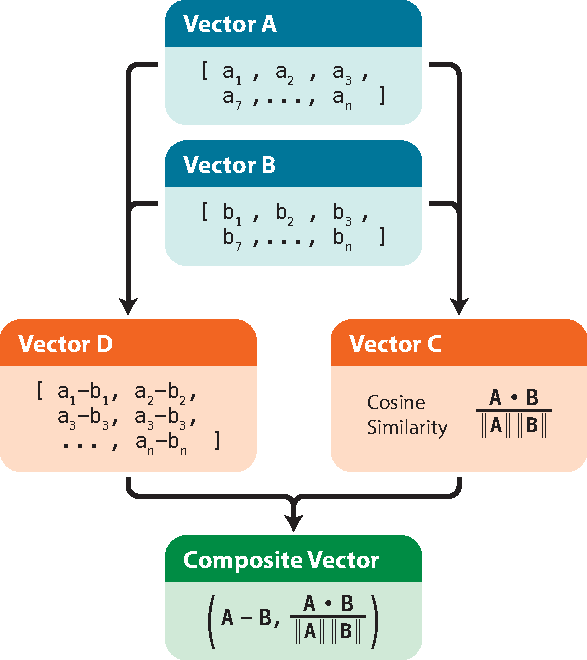
\includegraphics[width=0.9\textwidth]{composite_distance_vector_generation.pdf} % Placeholder for the graphic
%         \end{column}
%     \end{columns}
% \end{frame}

% % Step 3: Domain-Specific Fine-Tuning (Slide 3.5)
% \begin{frame}
%     \frametitle{Step 3: Domain-Specific Fine-Tuning}
    
%     General-purpose models lack the specialized ``vocabulary'' for academic text. To create a more discriminative embedding space, we fine-tune a pre-trained model on our course data using \textbf{deep metric learning}.
    
%     \fontsize{9}{9}\selectfont
%     \begin{columns}[T]
%         \begin{column}{0.55\textwidth}
%             \begin{alertblock}{Learning Objective: The Triplet Loss}
%                 We train the model using a \textbf{Triplet Loss} function, which teaches the model to understand nuanced similarity by operating on triplets of courses~\cite{Schroff_2015_CVPR, hermans2017defensetripletlossperson}:
%                 \begin{itemize}
%                     \item An \textbf{Anchor} course (\(A\))
%                     \item A \textbf{Positive}, equivalent course (\(P\))
%                     \item A \textbf{Negative}, non-equivalent course (\(N\))
%                 \end{itemize}
                
%                 \vspace{0.5em}
%                 The goal is to adjust the embedding space such that the distance between the Anchor and Positive is smaller than the distance between the Anchor and Negative, enforced by a margin (\(\alpha\)):
                
%                 \[ L(A, P, N) = \max\left(d(A, P) - d(A, N) + \alpha, 0\right) \]
%             \end{alertblock}
%         \end{column}
        
%         \begin{column}{0.4\textwidth}
%             \centering
%             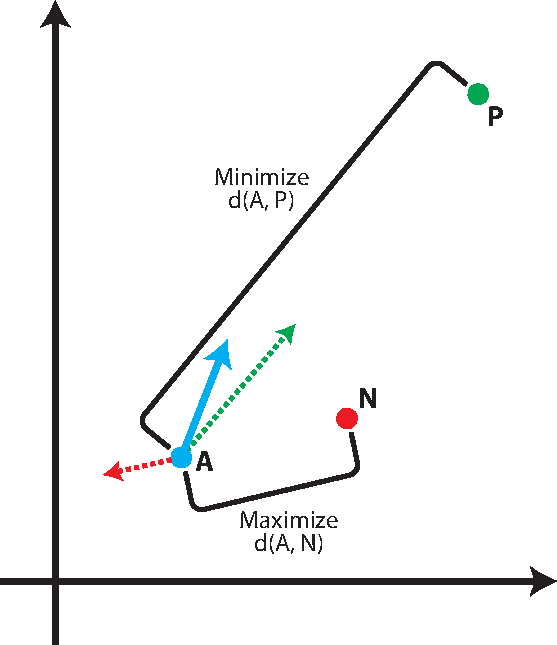
\includegraphics[width=0.8\textwidth]{tripletloss_viz_vertical.pdf} % Placeholder for the graphic
%         \end{column}
%     \end{columns}
% \end{frame}

% % Step 4: Downstream Classification (Slide 3.6)
% \begin{frame}
%     \frametitle{Step 4: Downstream Classification}
    
%     The final step is to feed the engineered composite distance vectors (\(\Delta_c\)) into a traditional machine learning model to produce the final equivalency prediction.
    
%     \begin{columns}[T]
%         \begin{column}{0.57\textwidth}
%             \hfill\vspace{3mm}
%             \begin{block}{Systematic Model Evaluation}
%                 To identify the most effective algorithm for this task, we systematically evaluated a comprehensive suite of models, including representatives from major algorithmic families:
%                 \begin{itemize}
%                     \item Linear Models (e.g., Logistic Regression)
%                     \item Kernel-Based Models (e.g., SVM)
%                     \item Instance-Based Models (e.g., KNN)
%                     \item Ensemble Models (e.g., Random Forest)
%                     \item Gradient Boosting (e.g., XGBoost)
%                 \end{itemize}
%             \end{block}
%         \end{column}
        
%         \begin{column}{0.38\textwidth}
%             \centering
%             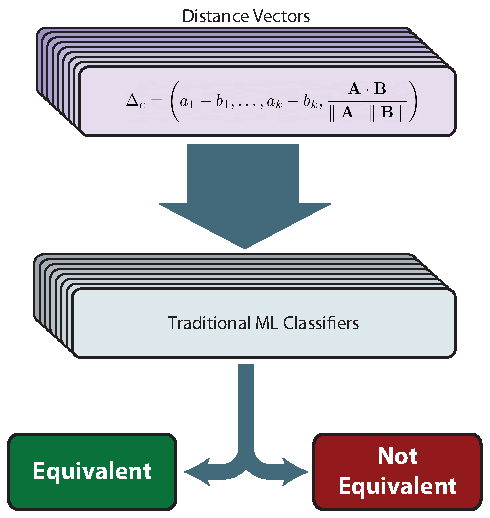
\includegraphics[width=\textwidth]{downstream_classification.pdf}
%         \end{column}
%     \end{columns}

%     \note[item]{The goal here was to find the best possible classifier for our specific feature vectors. By testing models from different families, we could probe the data for things like linear separability, complex non-linear decision boundaries, and feature interactions.}
%     \note[item]{The graphic on the right shows the simple version of this process: our feature vector goes in, the classifier makes a judgment, and a binary prediction comes out.}
%     \note[item]{The specific results of this competitive evaluation—that is, which models performed best—will be discussed in the upcoming Results section.}
    
% \end{frame}

% \section{Experimental Setup \& Results}
% \begin{frame}
%     \frametitle{Agenda}
%     \tableofcontents[currentsection]
% \end{frame}

% % Data & Evaluation (Slide 4.1)
% \begin{frame}
%     \frametitle{Datasets \& Evaluation}
    
%     The framework was trained and validated on a real-world dataset to ensure the results are robust and generalizable.
    
%     \vspace{2em}
%     \centering
%     \begin{tabularx}{0.95\textwidth}{>{\raggedright\arraybackslash}p{2.2cm} >{\raggedright\arraybackslash}X >{\raggedright\arraybackslash}X}
%         \toprule
%         \textbf{Characteristic} & \textbf{Initial Dataset}                                      
%         & \textbf{PPM Corpus}                                  \\
%         \midrule
%         \textbf{Source}         & Manually curated via ASSIST                   
%         & Program Pathways Mapper (PPM)                        \\
%         \addlinespace
%         \textbf{Purpose}        & Preliminary screening, prototyping, and initial classifier evaluation & Definitive fine-tuning and final pipeline evaluation \\
%         \addlinespace
%         \textbf{Ground Truth}   & Established articulation agreements                                   & Course Identification Number (C-ID)                  \\
%         \addlinespace
%         \textbf{Final Size}     & 400 course pairs (for evaluation set)                                 & 2,157 courses (across 157 classes)                   \\
%         \addlinespace
%         \textbf{Partitioning}   & Stratified random sample                                              & Stratified 50/50 train/test split                    \\
%         \bottomrule
%     \end{tabularx}

% \end{frame}

% % Finding 1: The Process & Rationale (Slide 4.2.1)
% \begin{frame}
%     \frametitle{Adapting a Model with Domain-Specific Fine-Tuning}
    
%     \begin{columns}[T]
%         \begin{column}{0.4\textwidth}
%             \hfill\vspace{2mm}
%             \begin{block}{The Process}
%                 We adapted a general-purpose model by fine-tuning it on the PPM Corpus using deep metric learning.
%                 \begin{itemize}
%                     \item \textbf{Objective:} Batch Triplet Loss functions were used to teach the model the nuanced semantics of academic text.
%                     \item \textbf{Optimization:} We paired a stable AdamW optimizer with a Cosine Annealing learning rate schedule to effectively navigate the complex loss landscape.
%                 \end{itemize}
%             \end{block}
%         \end{column}

%         \begin{column}{0.45\textwidth}
%             \centering
%             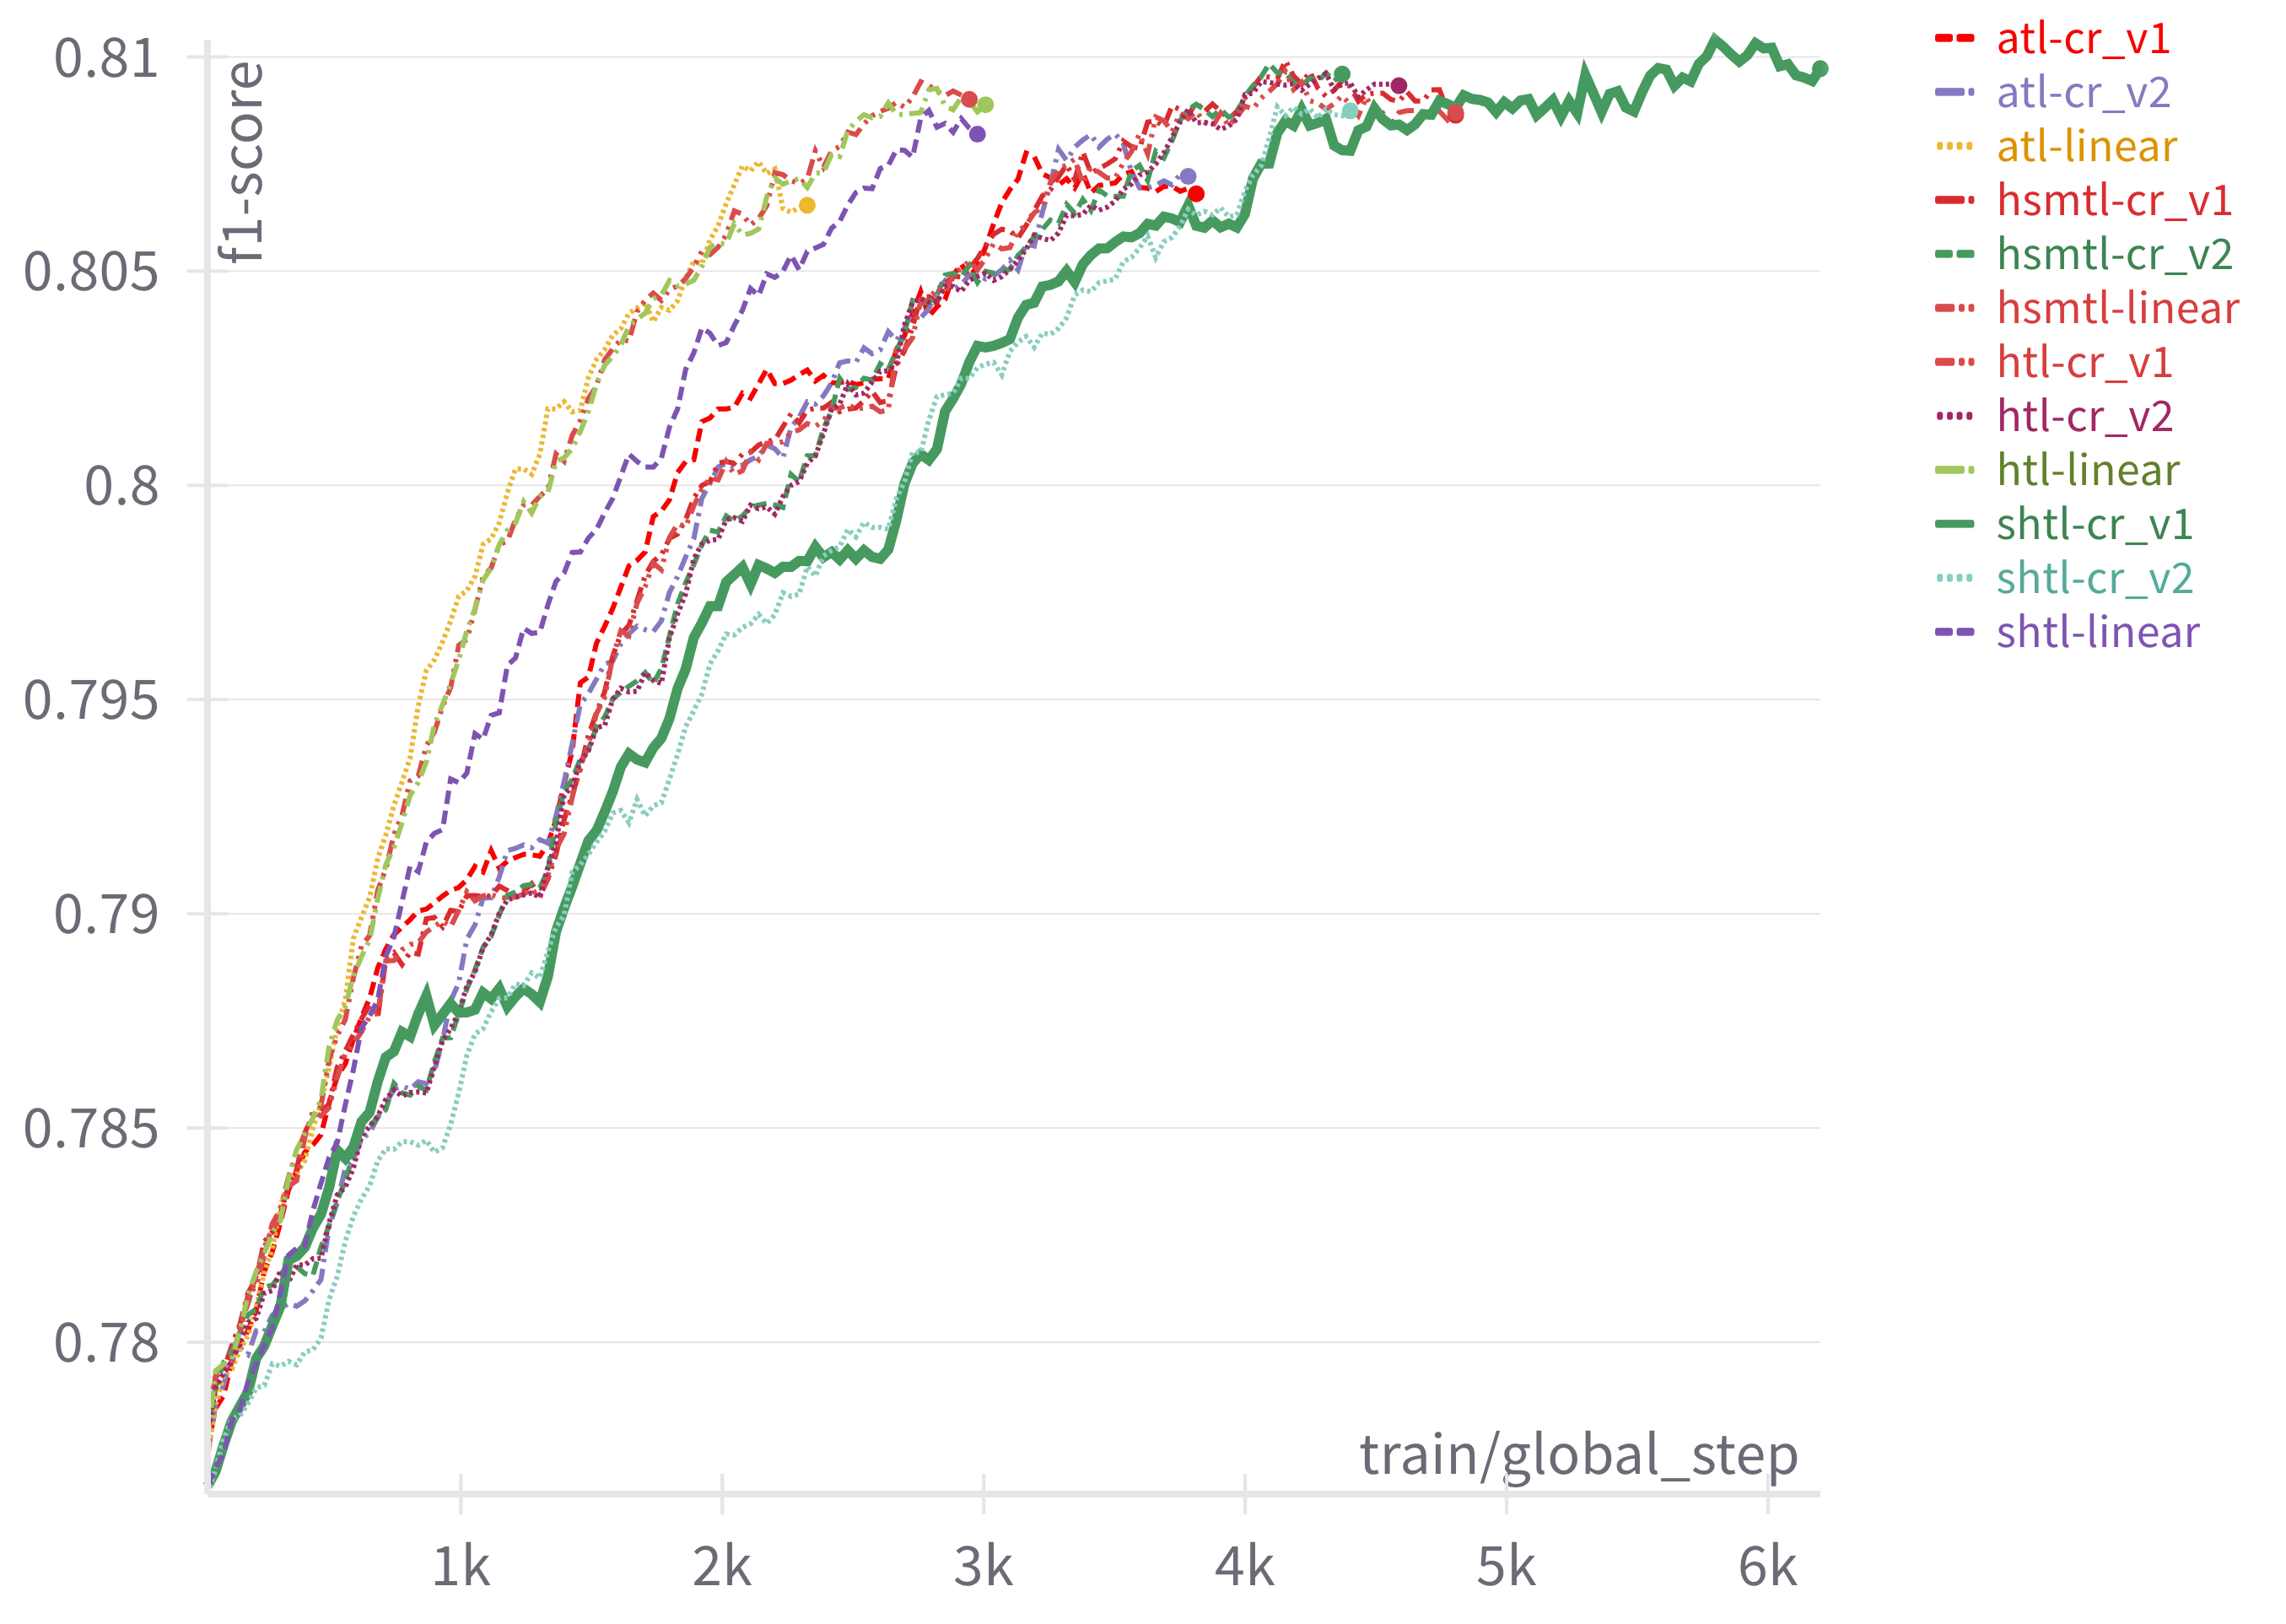
\includegraphics[width=\textwidth]{fine-tune_validation_f1_vs_step.png}
%             \vspace{2cm}
%             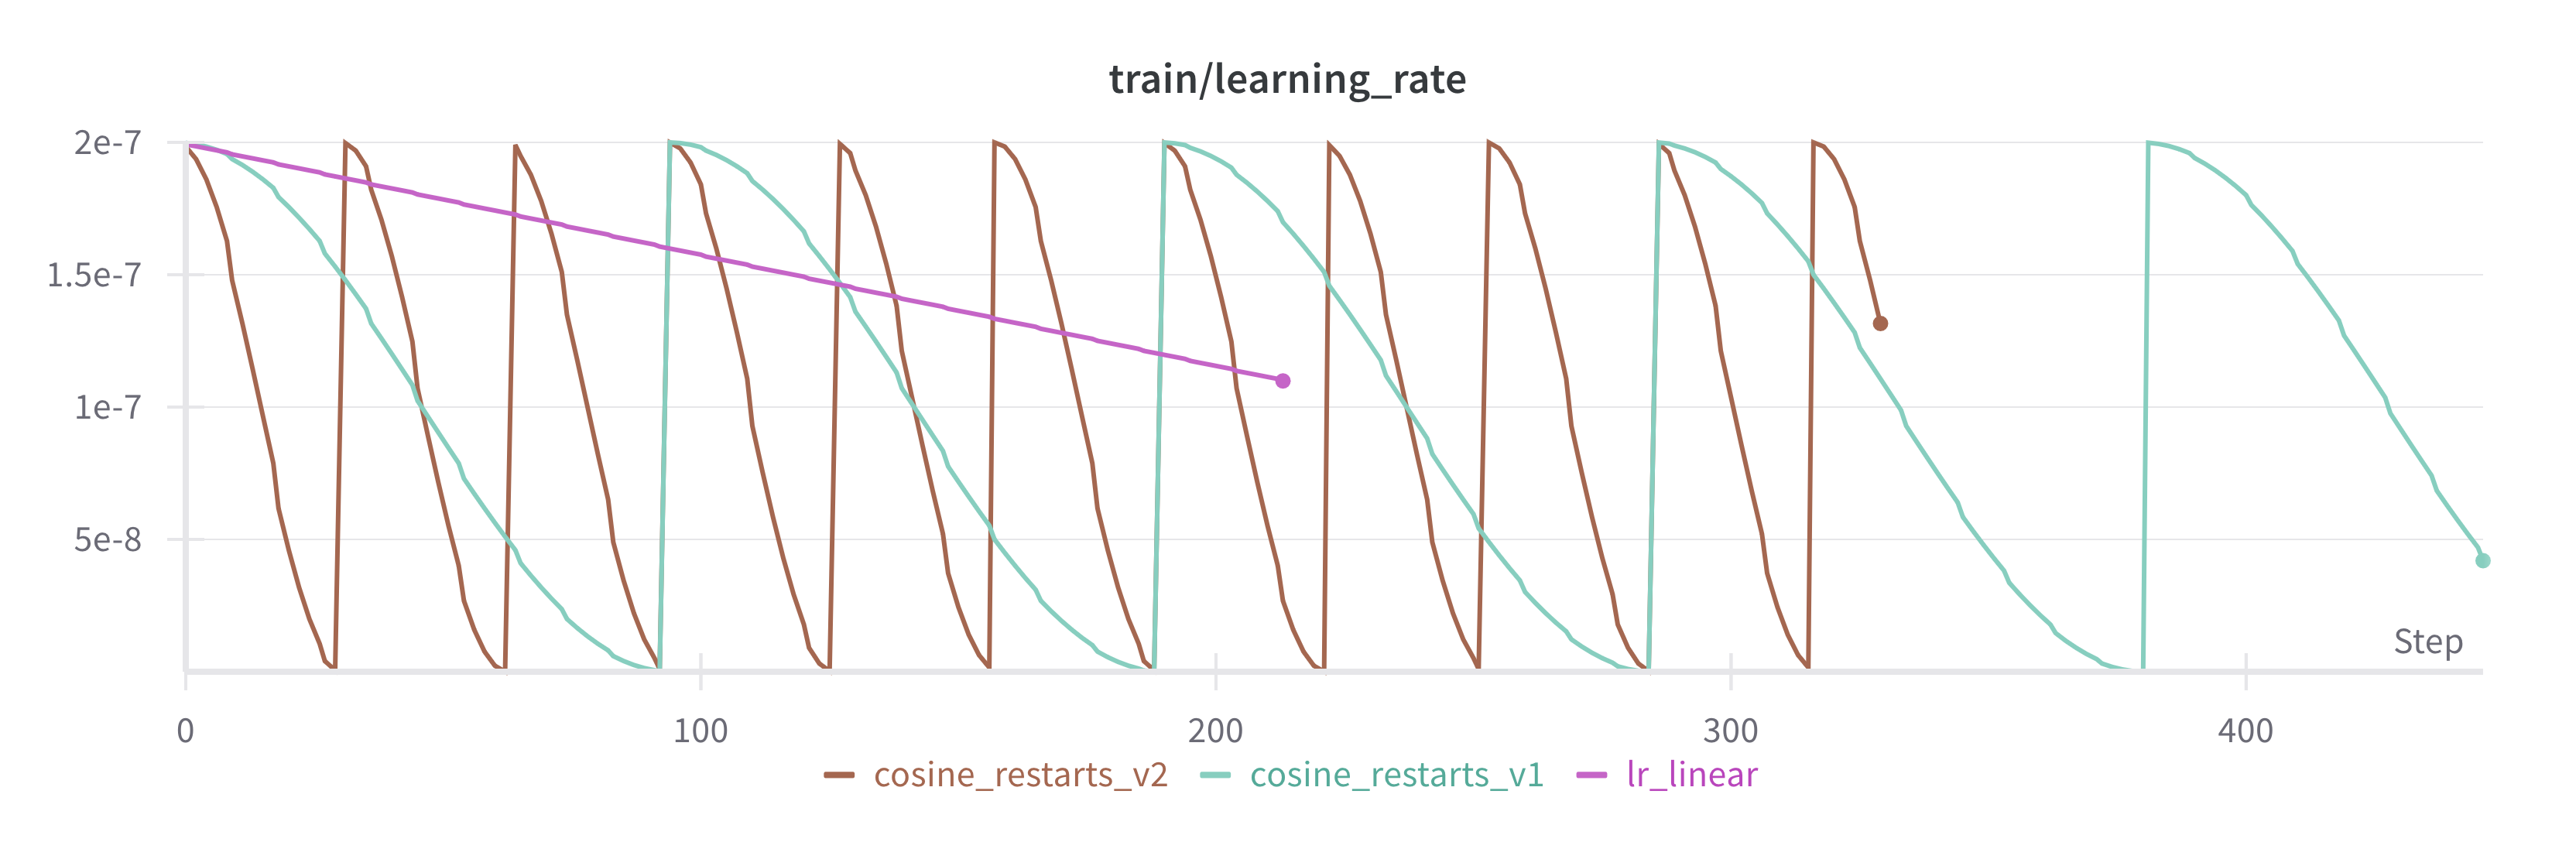
\includegraphics[width=0.95\textwidth]{learning rate.png}
            
%         \end{column}
%     \end{columns}
    
%     \note[item]{General-purpose models often miss the subtle but critical differences in academic language, so we needed to create a specialist.}
%     \note[item]{We used a Triplet Loss objective, which teaches the model to produce more discriminative embeddings for our specific task.}
%     \note[item]{The graph on the left shows the F1-score on a validation set improving as the model learns. The graph on the right shows the Cosine Annealing learning rate schedule we used, which helps the optimizer settle into a high-quality solution.}

% \end{frame}

% % Finding 1: The Result (The Punchline) (Slide 4.2.2)
% \begin{frame}
%     \frametitle{Finding 1: Fine-Tuned Model is Statistically Superior}
    
%     The result of the fine-tuning process is a model that is demonstrably more accurate and consistent on the held-out test data.
    
%     \begin{columns}[T]
%         \begin{column}{0.35\textwidth}
%             \begin{block}{Key Results}
%                 \begin{itemize}
%                     \item Our fine-tuned model (\textbf{bge-ft}) had the highest mean \(F_1\)-score (\(\mu=0.9786\)) and the lowest variance.
%                     \item A one-way ANOVA and Games-Howell post-hoc test confirmed that the performance gap is statistically significant against \emph{all} other models.
%                     \item This includes models that were orders of magnitude larger.
%                 \end{itemize}
%             \end{block}
%         \end{column}
        
%         \begin{column}{0.55\textwidth}
%             \centering
%             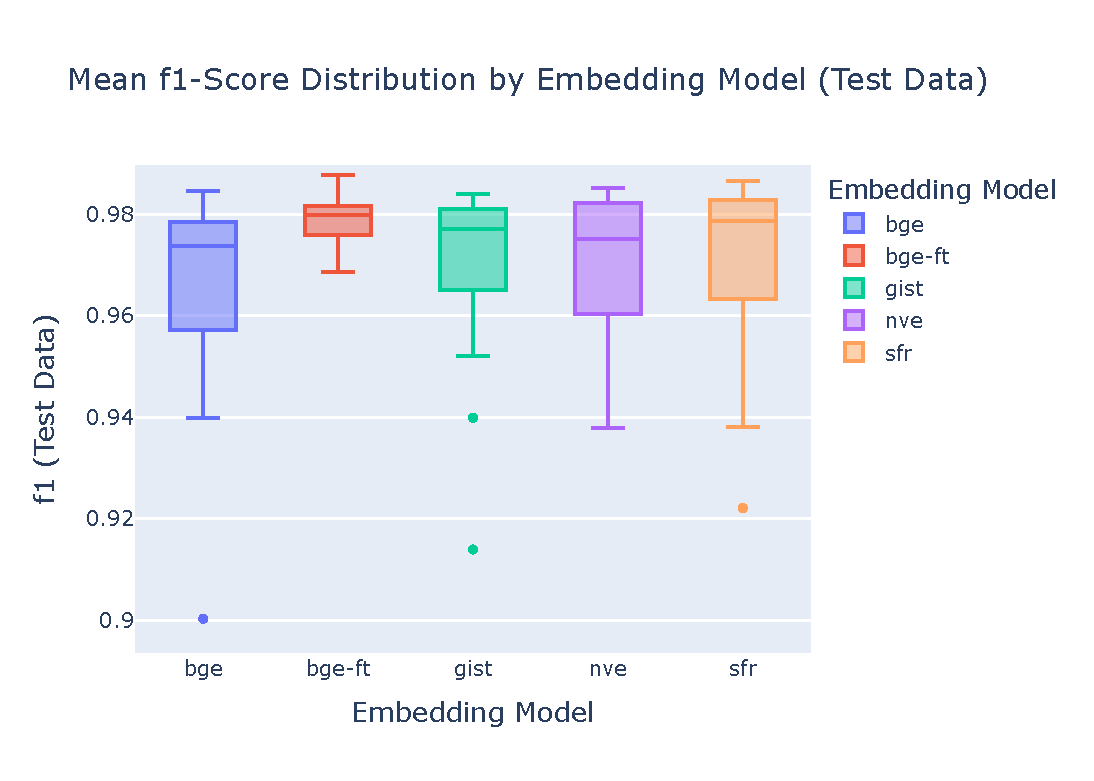
\includegraphics[width=\textwidth]{embeddingmodel_f1score_boxplot_test.pdf}
%         \end{column}
%     \end{columns}
    
%     \note[item]{This bar chart is the punchline. It compares the final F1 scores of our fine-tuned model, `bge-ft`, against its base version and other, much larger off-the-shelf models.}
%     \note[item]{As you can see, our model is the clear winner in terms of performance and consistency.}
%     \note[item]{This isn't just a small improvement; formal statistical tests (a one-way ANOVA and a Games-Howell post-hoc test) confirmed that this performance gap is statistically significant.}
% \end{frame}

% % Finding 1: The Insight (The "So What?") (Slide 4.2.3)
% \begin{frame}
%     \frametitle{Key Insight: Adaptation Outperforms Scale}
    
%     \begin{alertblock}{But ``So What?''}
%         For specialized domains like academic text, creating a bespoke embedding space through targeted fine-tuning is more effective than relying on sheer model scale.
%         \vspace{1em}
        
%         The fine-tuning process retrained the model's attention mechanism, teaching it the specific semantics required to make fine-grained distinctions that larger, general-purpose models may miss.
%     \end{alertblock}

%     \vfill
%     \centering
%     
\includegraphics[width=0.75\textwidth]{tuned_is_better.pdf}
    
%     \note[item]{This is the main takeaway from this finding. It answers the "so what?" question.}
%     \note[item]{A general-purpose model, even a huge one, might not understand the subtle but critical difference between a "survey" course, an "introductory" course, and a "foundations" course. Our model does.}
%     \note[item]{This is a key insight not just for this project, but for anyone working on NLP problems in specialized domains: targeted adaptation is crucial.}
% \end{frame}

% % Finding 2: All Finalists Perform Exceptionally Well (Slide 4.3.1)
% \begin{frame}
%     \frametitle{Finding 2: All Finalists Perform Exceptionally Well}
    
%     The first key result from the classifier evaluation is that our feature engineering and fine-tuning were highly effective, leading to exceptional performance across all finalist models.
    
%     \begin{columns}[T]
%         \begin{column}{0.35\textwidth}
%             \begin{block}{High \& Stable Performance}
%                 \begin{itemize}
%                     \item All four finalist classifiers (SVM, RF, XGBoost, KNN) achieved high and stable F1-scores.
%                     \item As the boxplot shows, the distributions are tightly clustered with mean scores approaching or exceeding \textbf{0.97}.
%                     \item This demonstrates the robustness of the upstream feature representation.
%                 \end{itemize}
%             \end{block}
%         \end{column}
        
%         \begin{column}{0.6\textwidth}
            
%             \centering
%             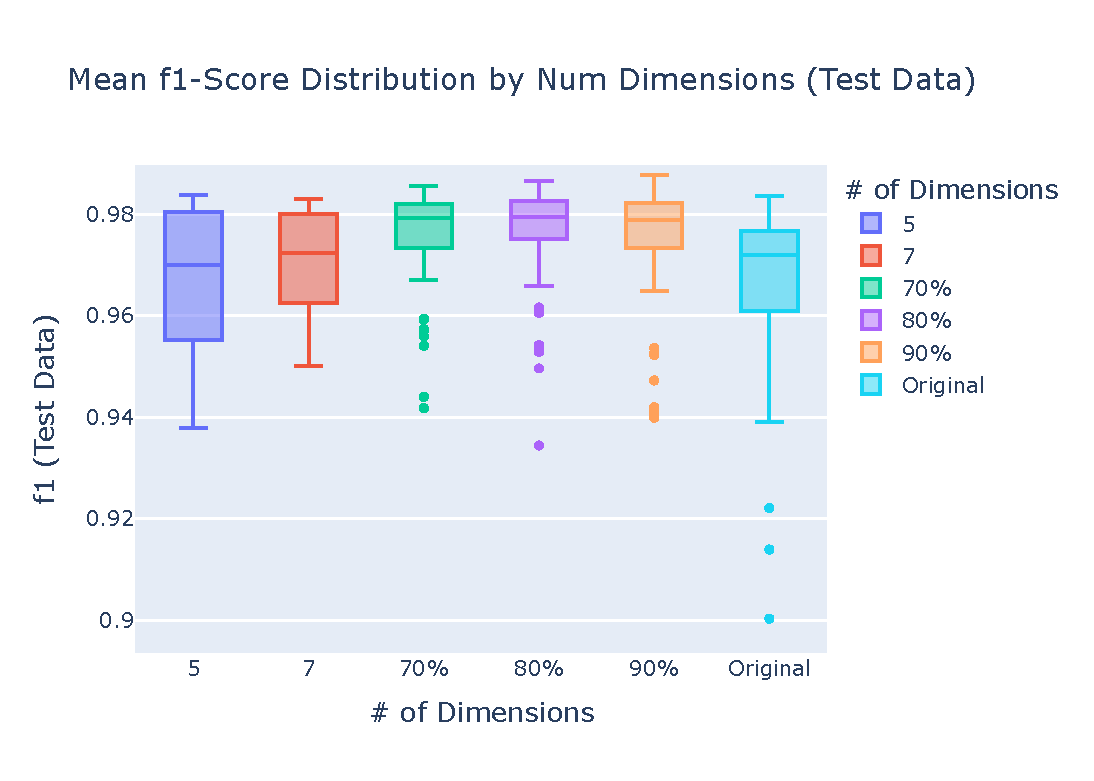
\includegraphics[width=\textwidth]{classifier_f1score_boxplot_test.pdf} % Placeholder for Figure 4.4
            
%         \end{column}
%     \end{columns}
    
%     \note[item]{The main message here is that our framework is successful. The features we created are so discriminative that any of the top-tier classifiers we chose for the final stage did an excellent job.}
%     \note[item]{This boxplot visualizes the F1-score distributions from our cross-validation on the test set. You can see how tightly grouped they are, all centered well above 0.97.}
%     \note[item]{This high baseline performance is a testament to the quality of the fine-tuned embeddings and the composite distance vector.}
    
% \end{frame}

% % Finding 2: The Accuracy vs. Efficiency Trade-Off (Slide 4.3.2)
% \begin{frame}
%     \frametitle{The Trade-Off: Peak Accuracy vs. Operational Efficiency}
    
%     While all models performed well, a deeper analysis reveals a classic trade-off, leading to context-dependent recommendations for deployment.
    
%     \begin{columns}[T]
%         \begin{column}{0.35\textwidth}
%             \begin{alertblock}{Key Finding}
%                 \begin{itemize}
%                     \item \textbf{For Maximum Accuracy:} The \textbf{Support Vector Machine (SVM)} was the statistical winner, proving to be the most accurate and consistent classifier.
                    
%                     \item \textbf{For Optimal Efficiency:} \textbf{Random Forest (RF) and XGBoost} were nearly as accurate but an order of magnitude faster and more predictable at inference time.
%                 \end{itemize}
%             \end{alertblock}
%         \end{column}
        
%         \begin{column}{0.6\textwidth}
            
%             \centering
%             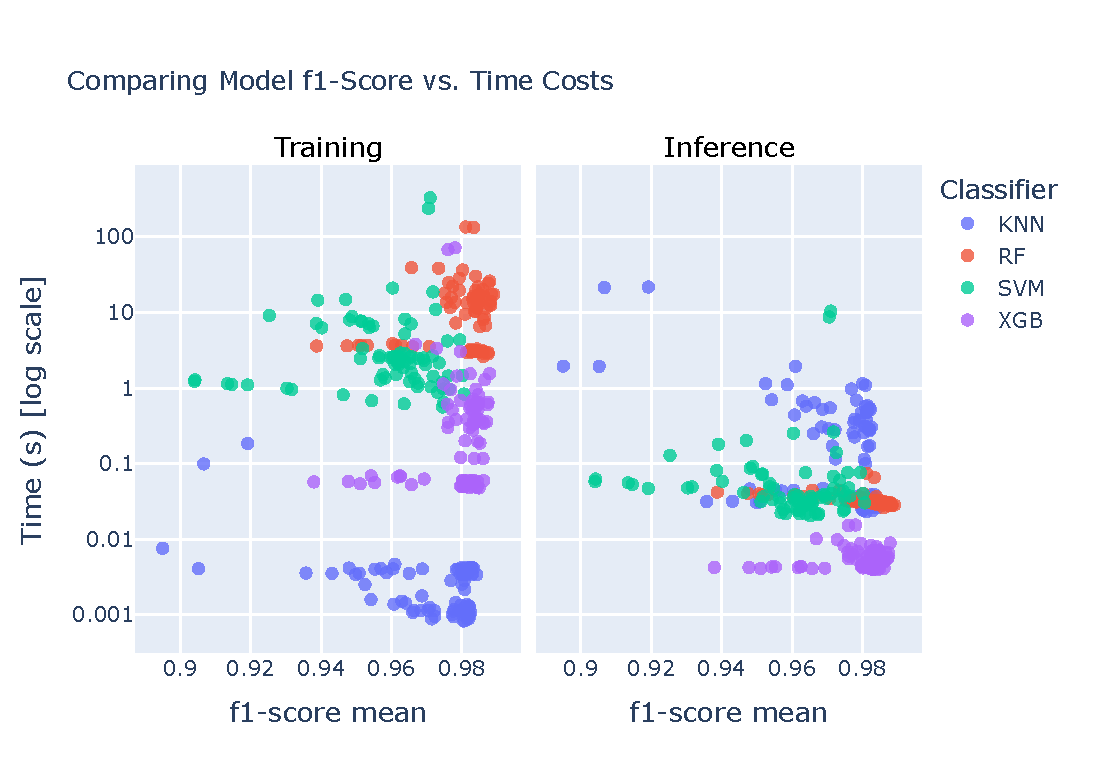
\includegraphics[width=\textwidth]{Model_Score_vs_Time_Costs.pdf} % Placeholder for Figure 4.3
            
%         \end{column}
%     \end{columns}
    
%     \note[item]{So, if all the models are good, which one should we choose? This scatterplot answers that question by showing accuracy versus inference speed.}
%     \note[item]{On the right, you can see that RF and XGBoost are incredibly fast, which is critical for a scalable, real-world system with many users.}
%     \note[item]{However, SVM, while slower, is statistically the most accurate. The choice depends on the deployment context: if you need the absolute highest accuracy, you choose SVM. If you need speed and scalability, you choose Random Forest or XGBoost.}
    
% \end{frame}

% \section{Qualitative Analysis: Beyond the Metrics}
% \begin{frame}
%     \frametitle{Agenda}
%     \tableofcontents[currentsection]
% \end{frame}

% % Why Do Errors Still Occur? (Slide 5.1)
% \begin{frame}
%     \frametitle{Qualitative Analysis: Why Do Errors Still Occur?}
    
%     High-level metrics don't tell the full story; a purely numerical analysis can be misleading~\cite{gauthier2022}.

%     \begin{columns}[T]
%         \begin{column}{0.5\textwidth}
%             \begin{alertblock}{Finding: The Bottleneck is Data, Not the Model}
%                 Our analysis revealed that most errors are not random, but are systematic issues rooted in the source data itself.
%                 \begin{itemize}
%                     \item A core set of \textbf{211 "hard" pairs} were misclassified by \textit{every single model} we evaluated.
%                     \vspace{1em}
%                     \item This proves the primary bottleneck for performance has shifted from being model-centric to \textbf{data-centric}.
%                 \end{itemize}
%             \end{alertblock}
%         \end{column}
        
%         \begin{column}{0.45\textwidth}
            
%             \centering
%             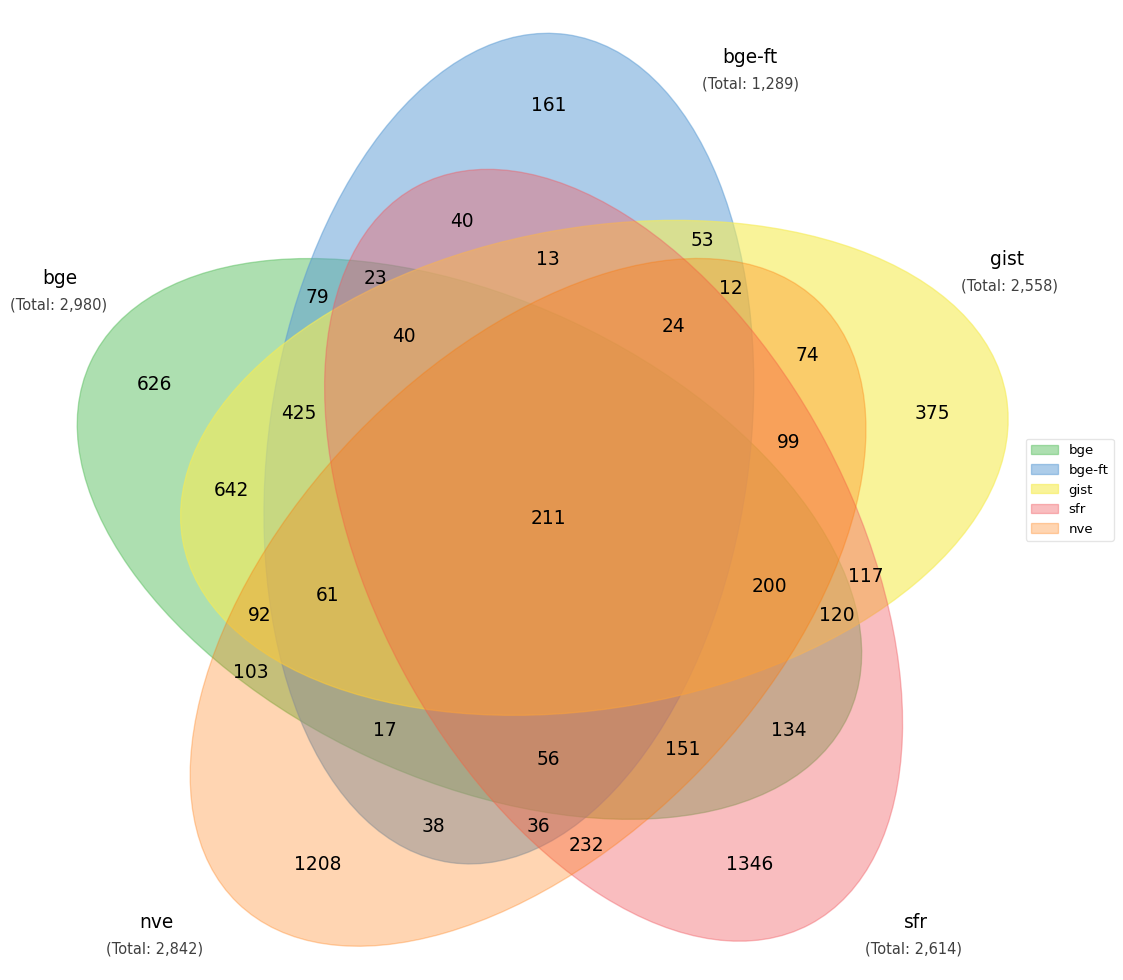
\includegraphics[width=\textwidth]{venn_with_totals_evaldata.png} % Placeholder for Figure 4.5
            
%         \end{column}
%     \end{columns}
    
%     \note[item]{The high degree of error overlap shown in the Venn diagram is critical. It shows that diverse models—from small specialists to large generalists—all failed on the exact same set of "hard" examples.}
%     \note[item]{This tells us the problem isn't idiosyncratic model weaknesses. The errors are systematic, pointing to inherent challenges in the source data itself.}
%     \note[item]{Therefore, the limiting factor is no longer model sophistication. The model often fails because the source data is ambiguous, inconsistent, or lacks a clear textual signal to support the ground-truth label.}
    
% \end{frame}

% % Shared Misclassifications (Slide 5.2)
% \begin{frame}
%     \frametitle{Shared Misclassifications: A Data-Centric Problem}
    
%     To diagnose the source of errors, we analyzed their overlap across all models. The results provide strong evidence that the errors are systematic.

%     \begin{columns}[T]
%         \begin{column}{0.5\textwidth}
%             \begin{block}{Failures are Systematic, Not Random}
%                 The analysis of misclassifications reveals a high degree of overlap across all evaluated models.
%                 \begin{itemize}
%                     \item A significant portion of failures are systematic products of the source data itself.
                    
%                     \item These "hard" examples consistently challenge a wide range of semantic models, from small specialists to large generalists.
                    
%                     \item This indicates errors stem from inherent data challenges—like ambiguity or annotation artifacts—not model weaknesses.
%                 \end{itemize}
%             \end{block}
%         \end{column}
        
%         \begin{column}{0.45\textwidth}
%             % --- SUGGESTED GRAPHIC ---
%             % The intersection bar chart from Figure 4.6 of the thesis
%             % would be the perfect graphic for this slide.
%             %
%             % It shows the high counts of shared errors across all
%             % model combinations, reinforcing the message that the
%             % failures are systematic.
%             %
%             % Title: "Number of Common Misclassified Pairs"
            
%             \centering
%             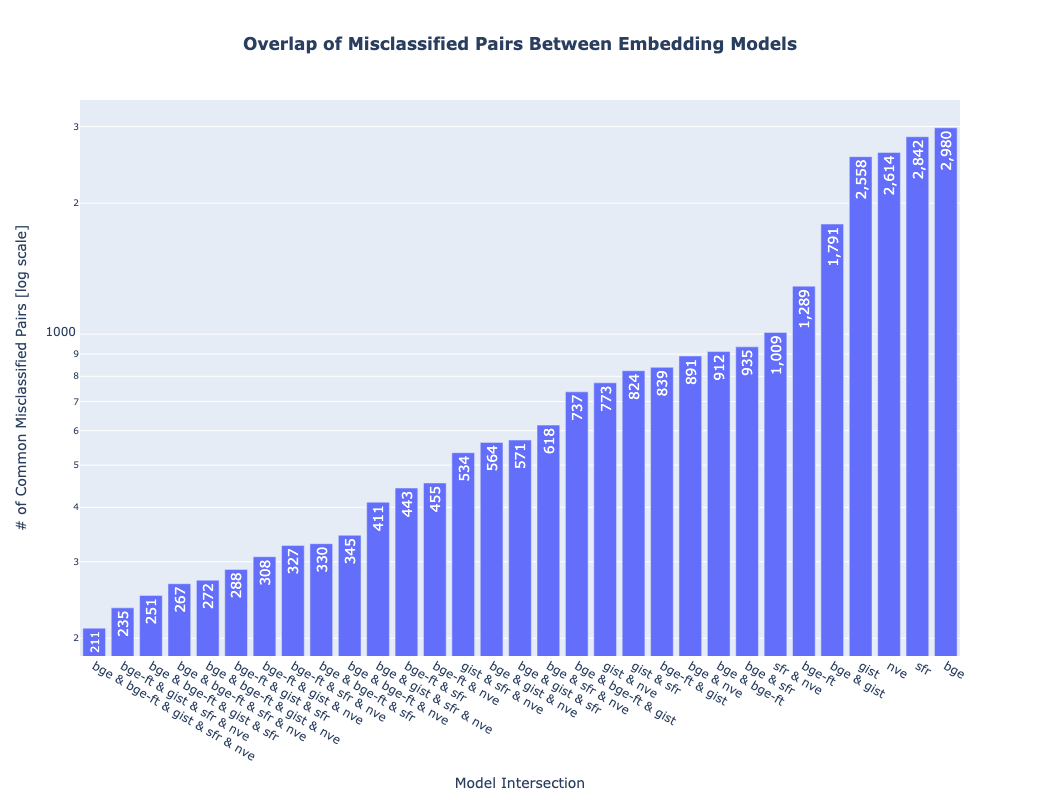
\includegraphics[width=\textwidth]{intersection_barchart_evaldata.png} % Placeholder for Figure 4.6
            
%         \end{column}
%     \end{columns}
    
%     \note[item]{This slide digs deeper into the "why" behind the errors. The key takeaway is that the models are largely agreeing with each other about which course pairs are difficult to classify.}
%     \note[item]{The bar chart on the right reinforces this, showing high counts of shared misclassified pairs between all combinations of the models we tested.}
%     \note[item]{This is strong evidence that the problem isn't the model's fault. In many cases, the models are correctly reporting that two course descriptions are not semantically similar. The issue is that the ground-truth label says they *should* be equivalent, pointing to an inconsistency in the source data itself.}

% \end{frame}

% % Root Cause Analysis: False Negatives (Slide 5.3.1)
% \begin{frame}
%     \frametitle{Root Cause Analysis: False Negatives (Missed Equivalencies)}
    
%     A False Negative occurs when the system fails to identify a true, existing equivalence. This represents a missed opportunity for a student.
    
%     \begin{columns}[T]
%         \begin{column}{0.43\textwidth}
%             \begin{block}{Causes}
%                 \begin{itemize}\vspace*{2mm}
%                     \item \textbf{Semantic Divergence:} Officially equivalent courses are described with vastly different terminology or pedagogical focus. The model correctly sees the texts as dissimilar; the error is in the inconsistent source data.
%                     \item \textbf{Minimalist Descriptions:} One or both course descriptions are too sparse or incomplete to provide enough textual signal for the model to find a confident match.\vspace*{2mm}
%                 \end{itemize}
%             \end{block}
%         \end{column}
%         \hfill
%         \begin{column}{0.51\textwidth}
%             % --- Example Table Graphic ---
%             \begin{alertblock}{Example: Semantic Divergence}
%                 \renewcommand{\arraystretch}{1.3}
%                 \begin{tabularx}{\textwidth}{>{\raggedright\arraybackslash}p{1.5cm}>{\raggedright\arraybackslash}X}
%                 \textbf{Course A} & \textit{"\dots examines\dots developmental milestones from middle childhood through adolescence\dots"} \\
%                 \textbf{Course B} & \textit{"\dots examines\dots diversity and inclusion\dots anti-bias curriculum\dots promote inclusive\dots classroom\dots"} \\
%                 \midrule
%                 \multicolumn{2}{c}{\textbf{Result:} False Negative} \\
%                 \multicolumn{2}{c}{(Model correctly sees texts as different)}
%                 \end{tabularx}
%             \end{alertblock}
%         \end{column}
%     \end{columns}

%     \note[item]{The first major error class is the False Negative, where our system misses a real equivalency. This could cause a student to unnecessarily retake a course.}
%     \note[item]{The example on the right is the most interesting cause. These two courses are both officially labeled with the same C-ID, making them equivalent. However, one is described using traditional developmental psychology language, while the other uses the language of social justice pedagogy.}
%     \note[item]{Our model correctly concludes that these two texts are not semantically similar. The failure here isn't in the model's understanding; it's in the inconsistency of the source data provided by the institutions.}
    
% \end{frame}

% % Root Cause Analysis: False Positives (Slide 5.3.2)
% \begin{frame}
%     \frametitle{Root Cause Analysis: False Positives (Incorrect Matches)}
    
%     A False Positive occurs when the system incorrectly classifies two non-equivalent courses as equivalent. This is a harmful error that could mislead a student.
    
%     \begin{columns}[T]
%         \begin{column}{0.43\textwidth}
%             \begin{block}{Causes}
%                 \begin{itemize}
%                     \item \textbf{Topical Overlap:} Courses cover the same broad subject but differ critically in academic level or their position in a sequence (e.g., Physics I vs. Physics II). The model correctly identifies high topical similarity but can't infer the sequence.
%                     \item \textbf{Vague Descriptions:} Descriptions use generic language, lacking the specific detail needed for differentiation. This is a known challenge in short-text semantic similarity~\cite{app13063911}.
%                 \end{itemize}
%             \end{block}
%         \end{column}
%         \hfill
%         \begin{column}{0.51\textwidth}
%             % --- Example Table Graphic ---
%             \begin{alertblock}{Example: Topical Overlap}
%                 \renewcommand{\arraystretch}{1.3}
%                 \begin{tabularx}{\textwidth}{>{\raggedright\arraybackslash}p{1.5cm}>{\raggedright\arraybackslash}X}
%                 \textbf{Course A} & PHYS-4A: \textit{"...a systematic introduction to the principles of classical mechanics..."} \\
%                 \textbf{Course B} & PHYS-4D: \textit{"...a systematic introduction to the principles of modern physics..."} \\
%                 \midrule
%                 \multicolumn{2}{c}{\textbf{Result:} False Positive} \\
%                 \multicolumn{2}{c}{(Model sees high topical overlap)}
%                 \end{tabularx}
%             \end{alertblock}
%         \end{column}
%     \end{columns}

%     \note[item]{The other major error class is the False Positive, where we incorrectly approve a pair. This is dangerous because it could lead a student to take a non-transferable course.}
%     \note[item]{The most common cause is topical overlap. For example, two physics courses at the same college. They are sequential, not equivalent.}
%     \note[item]{Because their descriptions both contain phrases like "systematic introduction to the principles of," the model sees high semantic overlap and makes an incorrect match. It cannot infer the sequential relationship from the text alone.}

% \end{frame}

% % The Primary Bottleneck (Slide 5.4)
% \begin{frame}
%     \frametitle{Conclusion of Analysis: The Primary Bottleneck}
    
%     The qualitative analysis leads to a critical insight regarding the future of automated articulation.
    
%     \begin{columns}[T]
%         \begin{column}{0.6\textwidth}
            
%             \begin{alertblock}{The Bottleneck has Shifted from Model-Centric to Data-Centric}
%                 With an optimized pipeline, the limiting factor may no longer be the model's architecture or semantic capability.
%                 \begin{itemize}
%                     \item The model is performing correctly; it accurately reports when two texts are not semantically similar.
%                     \item The remaining errors are artifacts of the source data itself: inconsistent descriptions, vague language, and information gaps.
%                     \item Therefore, the most promising path to further improvement lies not in novel architectures, but in methodologies that directly address the quality and consistency of the input data~\cite{gauthier2022}.
%                 \end{itemize}
%             \end{alertblock}
            
%         \end{column}
        
%         \begin{column}{0.35\textwidth}
%             \hfill\vspace{4mm}
            
%             \centering
%             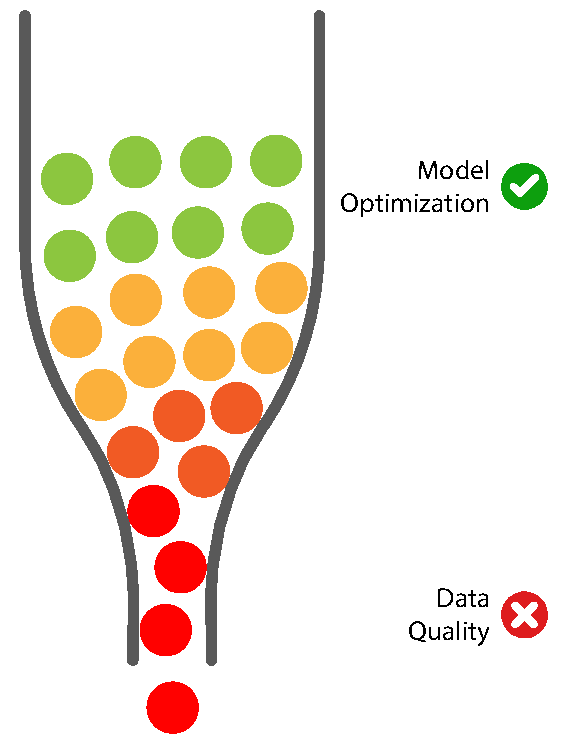
\includegraphics[width=0.8\textwidth]{data_quality_bottleneck.pdf}
            
%         \end{column}
%     \end{columns}

%     \note[item]{This slide presents the single most important conclusion from the entire qualitative analysis. After digging into why the model still makes mistakes, we arrived at this critical insight.}
%     \note[item]{To be clear on what this means: when the model is given two course descriptions that are written very differently, it correctly reports that they are not a good semantic match. The 'error' isn't in the model's logic, but in the ground-truth label that says they *should* be equivalent despite the textual evidence.}
%     \note[item]{Therefore, the problem has shifted. We've pushed the model's performance about as far as it can go with the current data. Simply using a bigger or more complex model is unlikely to resolve these data-inherent issues.}
%     \note[item]{This insight directly informs the future work for this project. The most promising path to further improvement lies not in novel model architectures, but in data-centric AI methodologies that focus on the quality and consistency of the input data.}
    
% \end{frame}

% \section{Conclusion}
% \begin{frame}
%     \frametitle{Agenda}
%     \tableofcontents[currentsection]
% \end{frame}

% % Limitations (Slide 6.1)
% \begin{frame}
%     \frametitle{Limitations}
    
%     While the proposed framework represents a significant advance, it is essential to acknowledge the boundaries of the current study.
    
%     \vspace{1mm}
%     \begin{block}{Key Limitations}
%         \hfill\vspace{-2mm}
%         \begin{columns}[T]
%             \begin{column}{0.3\textwidth}
%                 \textbf{Performance is Capped by Data Quality:}\\\vspace{1mm}
%                 The system's performance is fundamentally limited by the quality and content of the public course descriptions. It cannot infer information that is absent from vague, minimalist, or inconsistent source texts.
%             \end{column}
%             \hfill
%             \begin{column}{0.3\textwidth}
%                 \textbf{Generalizability of the Fine-Tuned Model:}\\\vspace{1mm}
%                 The specialized \textit{bge-ft} model was tuned on data from California's public colleges. Its performance may not be as high ``out-of-the-box'' in other contexts (e.g., private or non-US institutions) without re-tuning on local data.
%             \end{column}
%             \hfill
%             \begin{column}{0.3\textwidth}
%                 \textbf{Handling of Complex Articulation Rules:}\\\vspace{1mm}
%                 The framework simplifies articulation into a binary classification of course pairs and does not natively handle complex one-to-many or many-to-many agreements, a challenge that persists for many automated systems~\cite{pardos-articulation-2019}.
%             \end{column}
%         \end{columns}
%     \end{block}
    
% \end{frame}

% % Future Work (Slide 6.2)
% \begin{frame}
%     \frametitle{Future Work}
    
%     The findings and limitations of this study give rise to several promising avenues for future research.
    
%     \begin{columns}[T]
%         \begin{column}{0.45\textwidth}
%             \begin{block}{Key Research Directions}
%                 \begin{itemize}
%                     \item \textbf{Data-Centric AI Strategies:}  Focus on data quality via human-in-the-loop systems  and dynamic data augmentation.
%                     \item \textbf{Expanding Capabilities:}  Evolve the framework into a full course recommendation engine  and use graph-based methods for complex articulation rules.
%                     \item \textbf{Refinement of Current Work:}  Refine the core ML pipeline by exploring new feature combinations , multi-modal learning , and task-optimized loss functions.
%                 \end{itemize}
%             \end{block}
%         \end{column}
        
%         \begin{column}{0.5\textwidth}
            
%             \centering
%             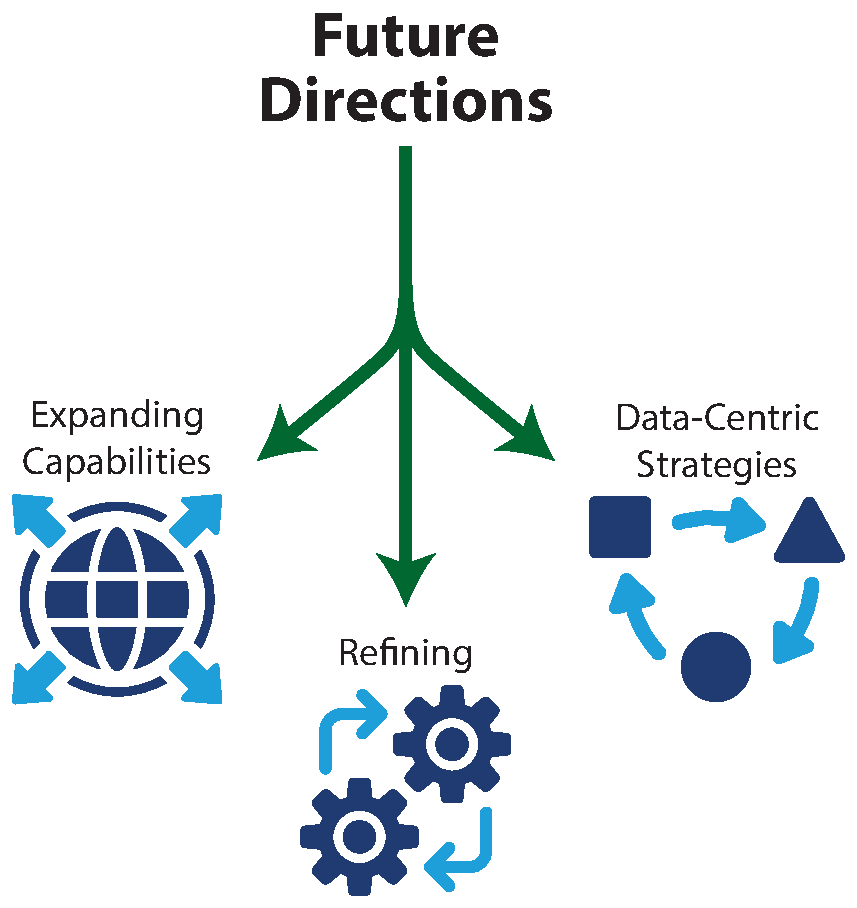
\includegraphics[width=0.75\textwidth]{future_directions.pdf}
            
%         \end{column}
%     \end{columns}
    
%     \note[item]{Given that data quality is the primary bottleneck , the most critical future work involves an interactive, human-in-the-loop system where an expert can review ambiguous pairs flagged by the model. We could also explore automatically requesting a more detailed syllabus if confidence is low.}
%     \note[item]{Active development is already underway to expand the framework into a full-scale course recommendation engine , which will eventually have a conversational interface. To handle complex one-to-many rules, another path is to model curricula as graphs and apply graph neural networks.}
%     \note[item]{Finally, there are opportunities to refine the core pipeline by investigating alternative composite distance measures , extending the model to analyze not just catalog descriptions but also the full text of syllabi or textbook lists , and exploring more sophisticated training methods like instruction-tuning.}
    
% \end{frame}

% % Summary of Contributions (Slide 6.3)
% \begin{frame}
%     \frametitle{Summary of Contributions}
    
%     This research confronted the challenge of manual course articulation by designing, developing, and validating a novel computational framework.

%     \vspace{3mm}
%     \begin{alertblock}{Primary Contributions}
%         \begin{enumerate}
%             \item \textbf{A Novel, Accurate, and Scalable Framework:} We developed an end-to-end pipeline that successfully automates course articulation using only public data, achieving state-of-the-art accuracy.
            
%             \item \textbf{Proof that Adaptation Outperforms Scale:} We proved that for this specialized domain, fine-tuning a smaller model for semantic nuance is statistically superior to relying on sheer model scale.
            
%             \item \textbf{A Practical Tool for Educational Equity:} We delivered a practical, computationally efficient, and privacy-preserving tool that can reduce administrative burden and help mitigate the systemic inequities faced by transfer students.
%         \end{enumerate}
%     \end{alertblock}
% \end{frame}

% \section{Wrap Up}

% % Thank You & Questions (Slide 7.1)
% \begin{frame}
%     \frametitle{} % No title for a clean look
%     \vfill % Vertically center the content
%     \centering
%     {\Huge \textbf{Thank You!!!}}\\
%     \vspace{5em}
%     {\Huge \textbf{Questions?}}
%     \vfill
% \end{frame}

% % Contact & Acknowledgments (Slide 7.2)
% \begin{frame}
%     \frametitle{Contact \& Acknowledgments}
%     \fontsize{9}{9}\selectfont
    
%     \begin{columns}[T]
%         \begin{column}{0.25\textwidth}
%             \begin{block}{Contact Information}
%                 \textbf{Mark S. Kim}
%                 \begin{itemize}
%                     \item \href{mailto:mkim22@mail.sfsu.edu}{mkim22@mail.sfsu.edu}
%                     % \item \href{https://www.linkedin.com/in/your-profile}{linkedin.com/in/your-profile}
%                     % \item \href{https://github.com/your-repo/project-name}{github.com/your-repo/project-name}
%                 \end{itemize}
%             \end{block}
%         \end{column}
        
%         \begin{column}{0.6\textwidth}
%             \begin{block}{Acknowledgments}
%                 I would like to express my deepest appreciation to:
%                 \begin{itemize}
%                     \item My advisors, Professors \textbf{Hui Yang}, \textbf{Arno Puder}, and \textbf{Anagha Kulkarni}, for their invaluable guidance and support.
%                     \item Professor \textbf{Tao He}, for the crucial suggestion to incorporate a global similarity metric into the feature vector.
%                     \item The \textbf{Program Pathways Mapper (PPM)} team for providing the foundational data for this work.
%                     \item The \textbf{SFSU Academic Technology Systems Team} for their support and the use of the POLARIS High-Performance Computing cluster.
%                 \end{itemize}
%             \end{block}
%         \end{column}
%     \end{columns}
% \end{frame}

% % This frame generates the bibliography at the end of the presentation.
% \begin{frame}[allowframebreaks]
%     \frametitle{References}
%     \printbibliography
% \end{frame}

\end{document}